\documentclass[12pt]{article}
\usepackage[english]{babel}
\usepackage{natbib}
\usepackage{url}
\usepackage[utf8x]{inputenc}
\usepackage{amsmath}
\usepackage{graphicx}
\graphicspath{{images/}}
\usepackage{parskip}
\usepackage{fancyhdr}
\usepackage{vmargin}
\setmarginsrb{3 cm}{2.5 cm}{3 cm}{2.5 cm}{1 cm}{1.5 cm}{1 cm}{1.5 cm}

\title{DOCTOR'S CHAMBER}								% Title
							


\makeatletter
\let\thetitle\@title

\let\thedate\@date
\makeatother

\pagestyle{fancy}
\fancyhf{}
\rhead{\theauthor}
\lhead{\thetitle}
\cfoot{\thepage}

\begin{document}

%%%%%%%%%%%%%%%%%%%%%%%%%%%%%%%%%%%%%%%%%%%%%%%%%%%%%%%%%%%%%%%%%%%%%%%%%%%%%%%%%%%%%%%%%

\begin{titlepage}
	\centering
    \vspace*{0.5 cm}
    
\includegraphics[scale = 0.35]{City-Logo.jpg}\\[1.0 cm]	% University Logo
    \textsc{\LARGE CITY UNIVERSITY}\\[2.0 cm]
    \textsc{\lARGE COMPUTER SCIENCE AND ENGINEERING}\\[0.2 cm]
    \textsc{\lARGE SYSTEM ANALYSIS AND DESIGN LABORATORY}\\[0.2 cm]
	\textsc{\Large CSE 326}\\[0.5 cm]				% Course Code
	\textsc{\large DESIGN AND DEVELOPMENT OF ONLINE DOCTOR APPOINTMENT ANDROID APPLICATION SYSTEM}\\[0.2 cm]
	\rule{\linewidth}{0.2 mm} \\[0.4 cm]
	{ \huge \bfseries \thetitle}\\
	\rule{\linewidth}{0.2 mm} \\[1.5 cm]
	
	\begin{minipage}{0.4\textwidth}
		
			\begin{flushright} \large
			\emph{STUDENT ID :} \\
			141352032\linebreak
			153402341\linebreak
			153402342\linebreak
			% Your Student Number
		\end{flushright}
	\end{minipage}\\[2 cm]
	
	{\large \thedate}\\[2 cm]
 
	\vfill
	
\end{titlepage}

%%%%%%%%%%%%%%%%%%%%%%%%%%%%%%%%%%%%%%%%%%%%%%%%%%%%%%%%%%%%%%%%%%%%%%%%%%%%%%%%%%%%%%%%%

\tableofcontents
\pagebreak

%%%%%%%%%%%%%%%%%%%%%%%%%%%%%%%%%%%%%%%%%%%%%%%%%%%%%%%%%%%%%%%%%%%%%%%%%%%%%%%%%%%%%%%%%

\textsc{\Large\section{BRAIN STORMING}}
\subsection{Smart Man Power Solution }
\textsc{\Small This Is An Android App. Its Abilities To Provide Dynamic, Disciplined And Dedicated Services In Labour Contract , Packaging Services , Security And Housekeeping.\cite{1}}

\subsection{Travel Guide Solution}
\textsc{\Small Use Travel Guide Solution App We Can Easily Travel One Place (Historical) To Another Place. We Can Easily Find Out Where Our Historical Place Situated. We Mark Where Our Historical Place Situated In Google Map, With Short Description.\cite{2}}

\subsection{Doctor's Chamber Information}
\textsc{\Small Here Our All Doctor’s Information Include. Individual All Doctor’s  Phone Number, Chamber, Which Specialist. Man Can Easily Find A Doctor Details. Its Very Helpful Our Society.}
\pagebreak











  

\textsc{\Large\section{ PRIORITY MATRIX}}


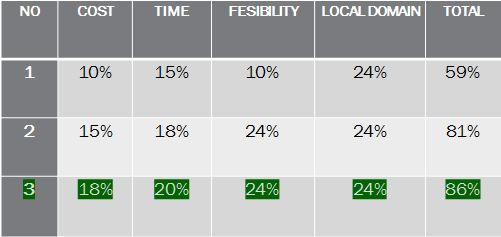
\includegraphics[scale = 0.99]{MAA.JPG}\\[1.0 cm]
\begin{center}
\caption{ Figure 1: Priority Matrix}
\end{center}


\section{PROJECT SELECTION}
{From Priority Matrix We Select Our Project}
\section*{DOCTOR’S CHAMBER INFORMATION}
\pagebreak


   
   
    


\section{CONCEPT MAPPING}


 
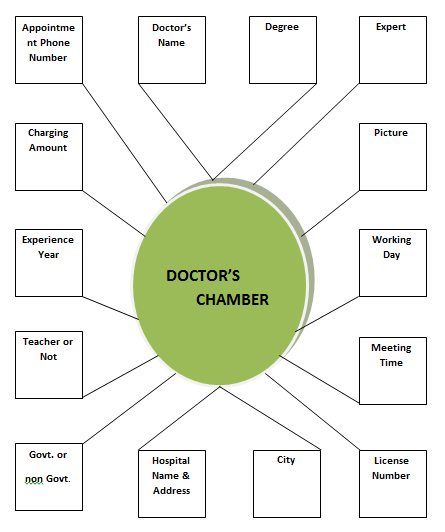
\includegraphics[height=7in]{Mapping.PNG}
\cite{3}
\begin{center}
 \caption{ Figure 2: Concept Mapping}
    
\end{center}

\newpage


\section{REQUIREMENT ANALYSIS}
\subsection {Hardware}\newline(i) Pc \newline(ii)Server Pc\newline (iii)Net 

\subsection {Software}\newline(i) Android Studio\newline (ii)Emulator\newline (iii)Java Run Time Environment\newline (iv) MySql\newline (v) Server Side Language(Php)\newline (v) Browser

\subsection {Other}\linebreak(i) Hospital Survey
\pagebreak


\section{STORY BOARDING}
\subsection{Before Using App}
Two Days Ago


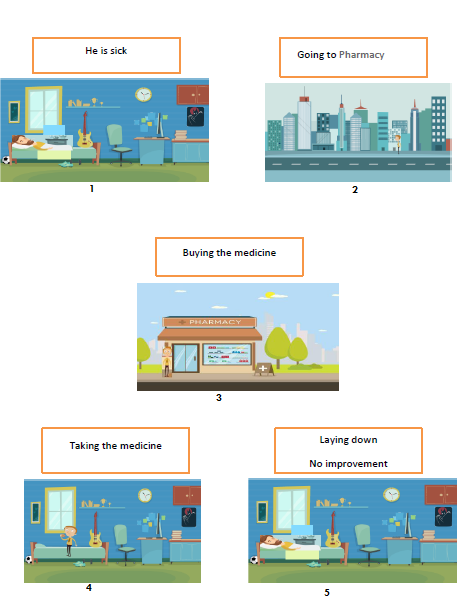
\includegraphics[scale = 0.99]{BEFORE1.PNG}\\[1.0 cm]

\pagebreak

\section*{Before Using App}
Previous Day

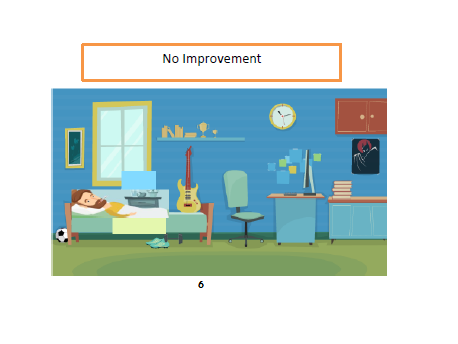
\includegraphics[scale = 0.99]{BEFORE2.PNG}\\[1.0 cm]
\pagebreak
\subsection{After Using App}
Present Day At Afternoon

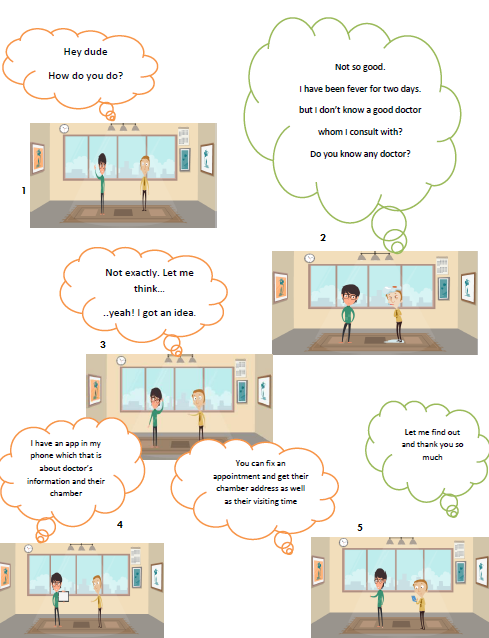
\includegraphics[scale = 0.99]{AFTER1.PNG}\\[1.0 cm]
\pagebreak
\section*{After Using App}
Next Day At Morning 

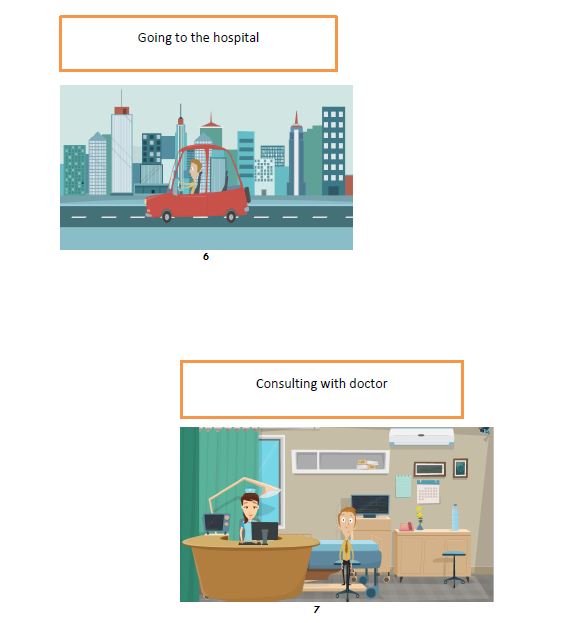
\includegraphics[scale = 0.99]{AFTER2.PNG}\\[1.0 cm]
\pagebreak
\section*{After Using App}
Same Day At Afternoon.......

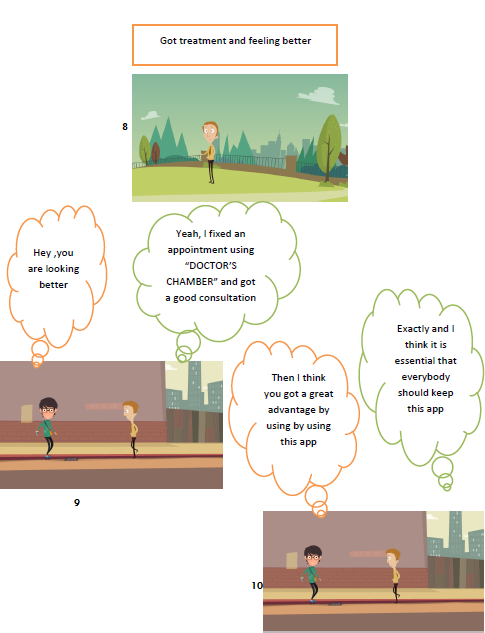
\includegraphics[scale = 0.99]{ATRER3.PNG}\\[1.0 cm]
\pagebreak
\section{PROTOTYPING}

\subsection{Log In App}

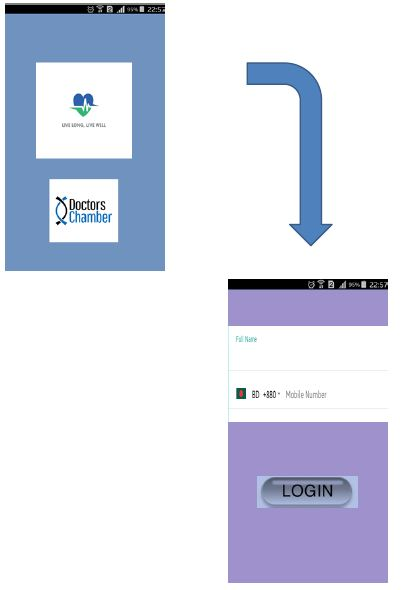
\includegraphics[scale = 0.99]{login.JPG}\\[1.0 cm]
\pagebreak

\subsection {Search By Specialist}

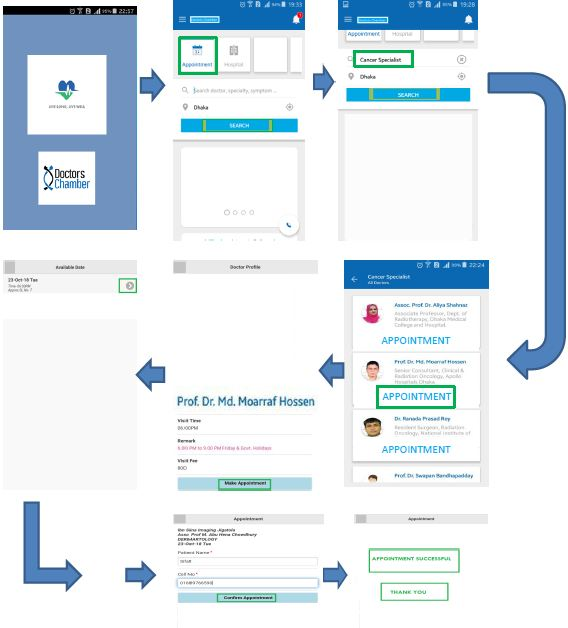
\includegraphics[scale = 0.99]{doctor.PNG}\\[1.0 cm]
\pagebreak

\subsection {Search By Hospital}

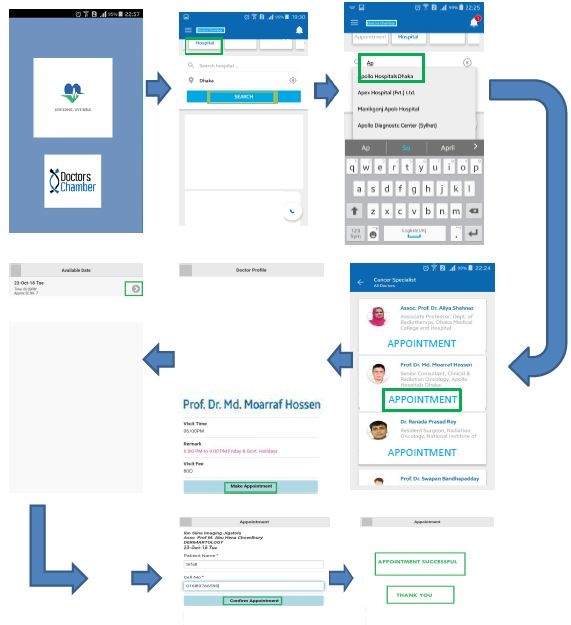
\includegraphics[scale = 0.99]{hospital.PNG}\\[1.0 cm]
\pagebreak
\section{USE CASE DIAGRAM}
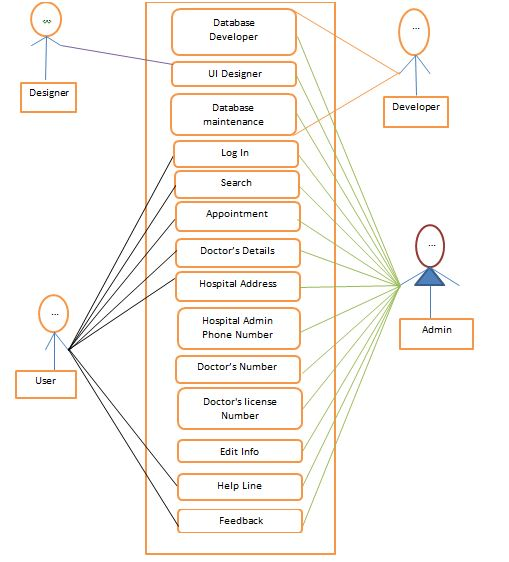
\includegraphics[height=18cm]{Use.PNG}
\begin{center}
 \caption{ Figure 3: Use Case Diagram}
    
\end{center}
\pagebreak
\section{SEQUENCE DIAGRAM}
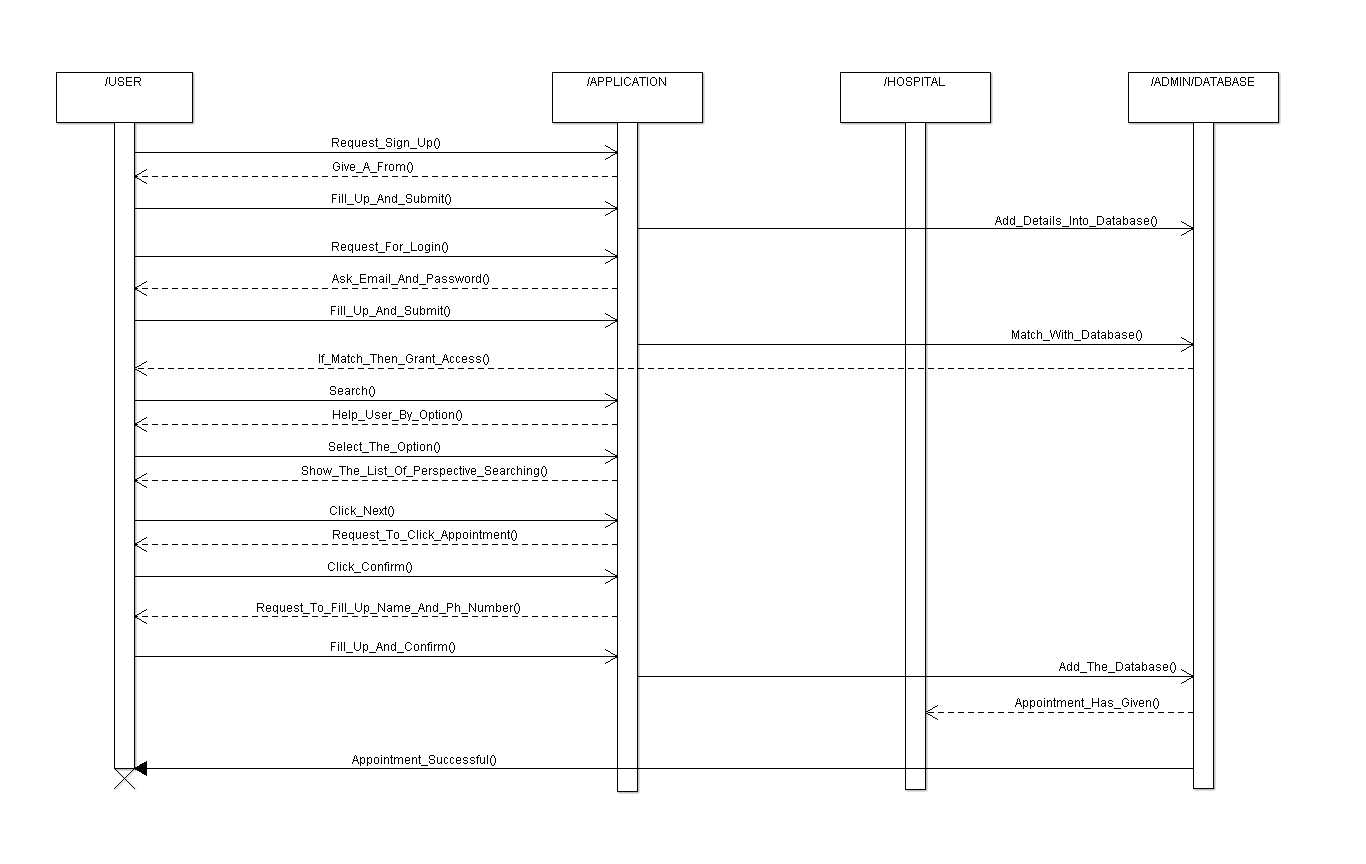
\includegraphics[height=11cm]{SequenceDiagram.PNG}
\begin{center}
 \caption{ Figure 4: Sequence Diagram}
    
\end{center}
\pagebreak
\section{DATABASE DESIGN}

\subsection{Full Table Of DataBase}

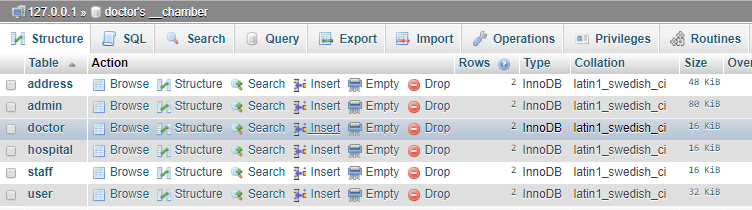
\includegraphics[scale = 0.68]{ALL.PNG}
\subsection{Doctor Table}

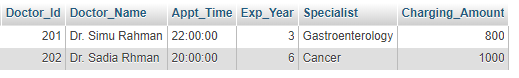
\includegraphics[scale = 0.99]{Tdoctor.PNG}

\subsection{Hospital Table}

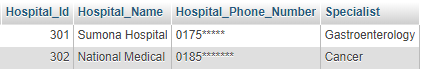
\includegraphics[scale = 0.99]{Thospital.PNG}

\subsection{User Table}

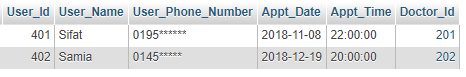
\includegraphics[scale = 0.99]{Tuser.PNG}


\subsection{Address Table}

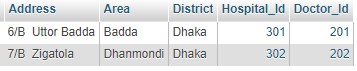
\includegraphics[scale = 0.99]{TADD.PNG}

\subsection{Admin Table}

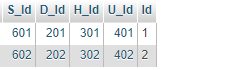
\includegraphics[scale = 0.99]{Tadmin.PNG}

\subsection{Staff Table}

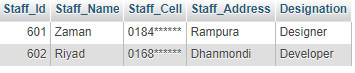
\includegraphics[scale = 0.99]{Tstaff.PNG}


\pagebreak

\section{DATA BASE SCHEMA}

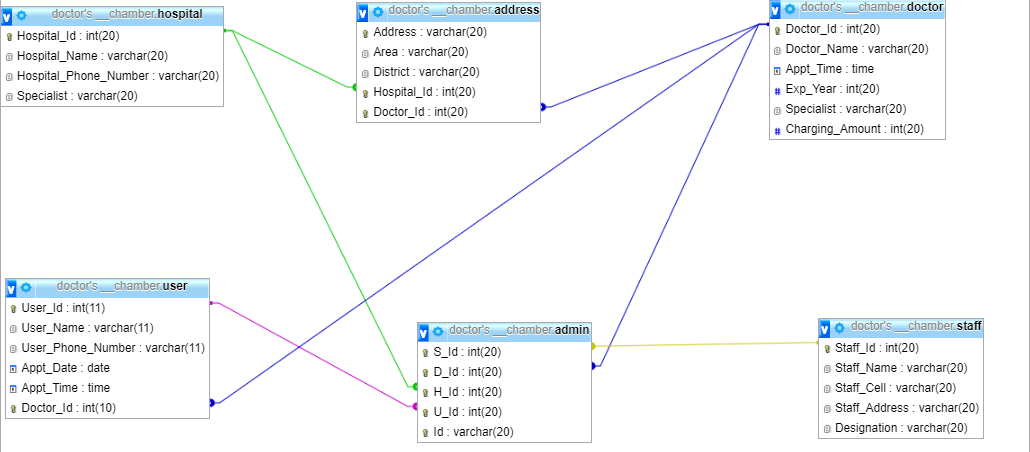
\includegraphics[height=6cm]{ER.PNG}
\begin{center}
 \caption{ Figure 5: Data Base Schema}
    
\end{center}

\section{DATA FLOW DIAGRAM}

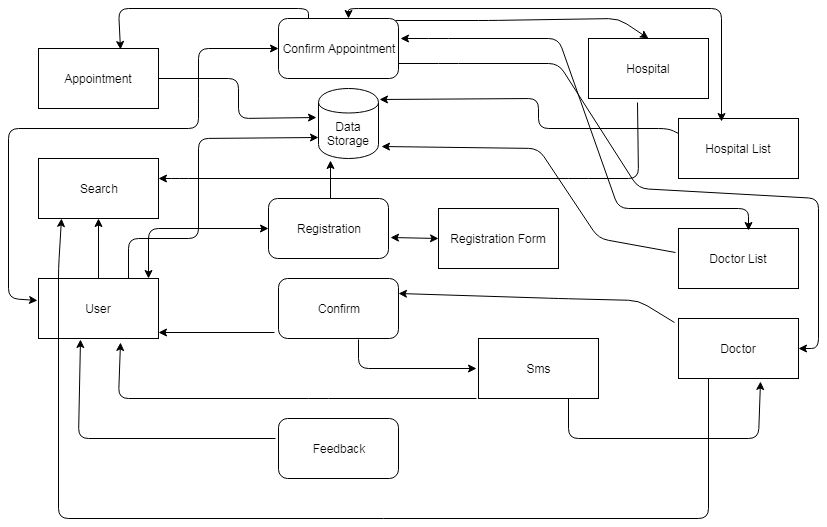
\includegraphics[height=9cm]{Dataflow.png}
\begin{center}
 \caption{ Figure 6: Data Flow Diagram}
    
\end{center}

\pagebreak

\section{ER DIAGRAM}

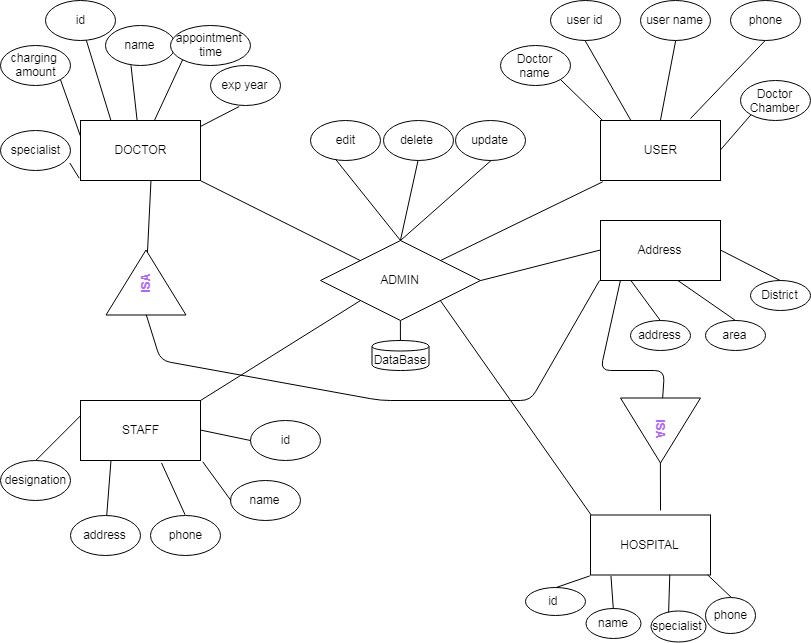
\includegraphics[scale = 0.45]{EE.jpg}\\[8.0 cm]
\begin{center}
 \caption{ Figure 7: Er Diagram}
    
\end{center}

\pagebreak

\section{ACTIVITY DIAGRAM}

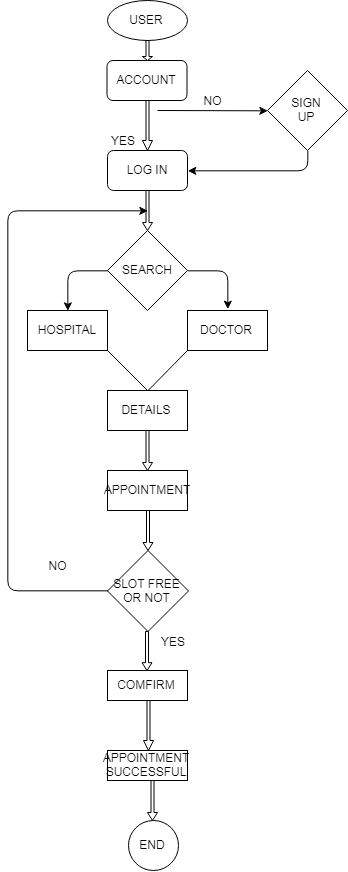
\includegraphics[height=7in]{ActivityDiagram.png}
\begin{center}
 \caption{ Figure 8: Activity Diagram}
    
\end{center}



\begin{thebibliography}{99}
 

\bibitem{1} \url{https://en.wikipedia.org/wiki/ManpowerGroup}
\bibitem{2} \url{https://en.wikipedia.org/wiki/Guide_book}

\bibitem{3} \url{https://en.wikipedia.org/wiki/Concept_map}

\end{thebibliography}




\end{document}